\documentclass[11pt, oneside]{article}   	% use "amsart" instead of "article" for AMSLaTeX format
\usepackage{geometry}                		% See geometry.pdf to learn the layout options. There are lots.
\geometry{letterpaper}  
\usepackage{graphicx}  
\usepackage{amsmath,amsthm,amssymb,amsfonts}                		% ... or a4paper or a5paper or ... 
%\geometry{landscape}                		% Activate for rotated page geometry
%\usepackage[parfill]{parskip}    		% Activate to begin paragraphs with an empty line rather than an indent
\usepackage{graphicx}				% Use pdf, png, jpg, or eps§ with pdflatex; use eps in DVI mode
								% TeX will automatically convert eps --> pdf in pdflatex		
\usepackage{amssymb}

%SetFonts

%SetFonts


\title{Data analysis of red wine quality}
\author{Xiaolan Yuan}
%\date{}							% Activate to display a given date or no date

\begin{document}
\maketitle
\section{Brief introduction}
To find the factors that highly impact the quality of red wines, we conduct an analysis of a dataset consisting of 11 different types of information of 1599 sample red wines. The information contains: `fixed acidity',`volatile acidity',`citric acidity',`residual sugar',`chlorides',`free sulfur dioxide',`total sulfur dioxide',`density',`pH',`sulphates' and `alcohol'. The quality of the a red wine is represented as a integer ranged from 0(low) to 10(high).\\
\\
%Our aim is to select the smallest number of candidate predictors which have strong influence on the quality level of red wine. In order to do that, we need to simplify the training dataset by delete the predictors which are highly linked to others. It means that if we have several highly linked predictors, we can just choose one of them to fit our model.
In this article, we will use the linear regression with multiple variables to accomplish our analysis.
\section{Analyze the correlation among candidate predictors}
By computing the correlation matrix of all predictors, we can determine if two predictors are highly correlated or not. Here we denote two predictors as highly correlated if the absolute value of the corresponding correlation coefficient for these two predictors is greater than or equal to 0.5. Otherwise, we consider that there is no significant link between these two predictors.
\begin{table}[!ht]
\centering
\begin{tabular}{rrrrrrrrrrrr}
  \hline
 & f.a & v.a. & c.a. & r.s. & chlo. & f.s.d. & t.s.d & dens. & pH & sul. & alco. \\ 
  \hline
f.a & 1.00 & -0.26 & 0.67 & 0.11 & 0.09 & -0.15 & -0.11 & 0.67 & -0.68 & 0.18 & -0.06 \\ 
  v.a. & -0.26 & 1.00 & -0.55 & 0.00 & 0.06 & -0.01 & 0.08 & 0.02 & 0.23 & -0.26 & -0.20 \\ 
  c.a. & 0.67 & -0.55 & 1.00 & 0.14 & 0.20 & -0.06 & 0.04 & 0.36 & -0.54 & 0.31 & 0.11 \\ 
  r.s. & 0.11 & 0.00 & 0.14 & 1.00 & 0.06 & 0.19 & 0.20 & 0.36 & -0.09 & 0.01 & 0.04 \\ 
  chlo. & 0.09 & 0.06 & 0.20 & 0.06 & 1.00 & 0.01 & 0.05 & 0.20 & -0.27 & 0.37 & -0.22 \\ 
  f.s.d. & -0.15 & -0.01 & -0.06 & 0.19 & 0.01 & 1.00 & 0.67 & -0.02 & 0.07 & 0.05 & -0.07 \\ 
  t.s.d & -0.11 & 0.08 & 0.04 & 0.20 & 0.05 & 0.67 & 1.00 & 0.07 & -0.07 & 0.04 & -0.21 \\ 
  dens. & 0.67 & 0.02 & 0.36 & 0.36 & 0.20 & -0.02 & 0.07 & 1.00 & -0.34 & 0.15 & -0.50 \\ 
  pH & -0.68 & 0.23 & -0.54 & -0.09 & -0.27 & 0.07 & -0.07 & -0.34 & 1.00 & -0.20 & 0.21 \\ 
  sul. & 0.18 & -0.26 & 0.31 & 0.01 & 0.37 & 0.05 & 0.04 & 0.15 & -0.20 & 1.00 & 0.09 \\ 
  alco. & -0.06 & -0.20 & 0.11 & 0.04 & -0.22 & -0.07 & -0.21 & -0.50 & 0.21 & 0.09 & 1.00 \\ 
   \hline
\end{tabular}
\caption{The correlation matrix of the 11 candidate predictors}
\end{table}
%%%%%%%%%%%%%
%problem 1
%%%%%%%%%%%%%
\subsection{Find highly correlated predictors}
The correlation matrix for the 11 initial candidate predictors above is demonstrated in Table 1. By the observation, we can get the result:(If two predictor are correlated, we will only mention it once.)
\begin{itemize}
\item `fixed acidity' is highly correlated to `citric acidity', `density', and 'pH' with coefficients 0.67, 0.67, and -0.68 respectively.
\item `citric acidity' is highly correlated to `volatile acidity' and `pH' with coefficient -0.55 and -0.54.
\item `free sulfur dioxide' is highly correlated to `total sulfur dioxide' with coefficient 0.67
\item  `density' is highly correlated to `alcohol' with coefficient -0.5
\end{itemize}
%%%%%%%%%%%%%
%Problem 2
%%%%%%%%%%%%%
\subsection{Data transform}
In order to determine if we need to transform the response, we need to use the 11 predictors to conduct a multiple linear regression. The residuals of the regression are shown in the figure as follows:
\begin{figure}[!htbp] 
\centering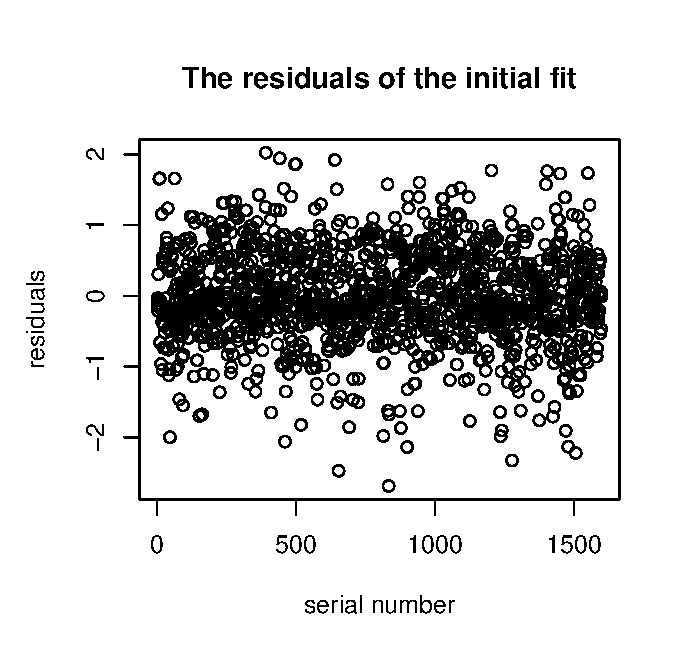
\includegraphics[width=2in]{fit0residuals.eps}  
\end{figure}
\\ 
As we can see, the residuals of the multiple linear regression are random distributed and the values of residuals are similar to each other. Therefore, there is no need to transform the response value (quality level). 
%%%%%%%%%%%%%
%Problem 3
%%%%%%%%%%%%%
\subsection{Analyze three predictors for measuring acidity}
In this dataset, we have 3 predictors that measure acidity: $X_1$: `fixed acidity', $X_2$: `volatile acidity', and $X_3$: `citric acidity'. By the analysis above, we know that `citric acidity' is the only one of them that highly correlated to both of the others. So, if we want to choose one of them as the predictor $A_1$ to replace all of them, we should choose $X_3$ (citric acidity).
%%%%%%%%%%%%%
%Problem 4
%%%%%%%%%%%%%
\subsection{Three predictor related to sulfur}
In this dataset, we have 3 predictors related to sulfur literally: `free sulfur dioxide',`total sulfur dioxide' and `sulphates'. By Table 1 we can observe that only the first two are highly correlated to each other, but `sulphates' almost has no correlation with them. So it is not wise to only choose one predictor among them.
%%%%%%%%%%%%%
%Problem 5
%%%%%%%%%%%%%
\subsection{Dichotomize the variable `density'}
By the scatterplot of the variable `density', we can do a dichotomization of the dataset as follows in the figure.
\begin{figure}[!htbp] 
\centering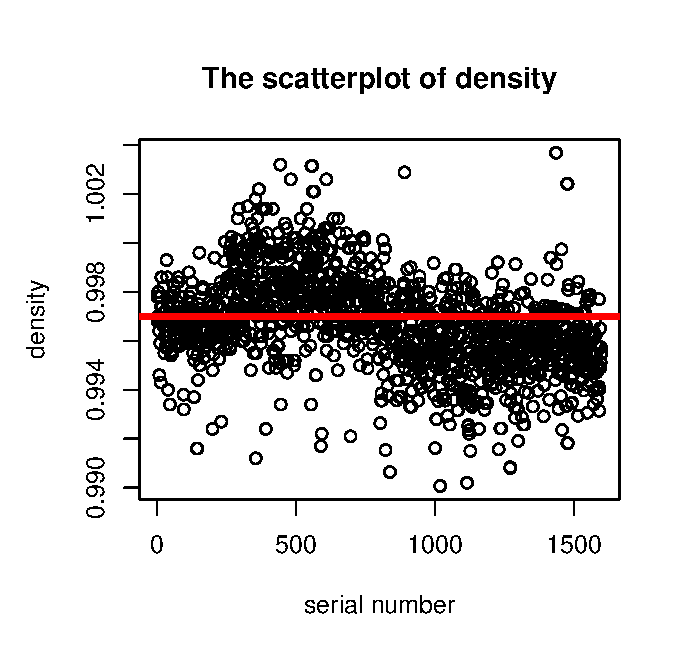
\includegraphics[width=2in]{density.eps}  
\end{figure}
\\
The red line here is $y=0.997$. Then we define $D$ as a new variable to show `density':
\begin{equation}
D_i=
\left\{
\begin{aligned}
&1,\qquad\text{if the i-th density is greater than or equal to 0.997}\\
&0,\qquad\text{if the i-th density is less than 0.997}
\end{aligned}
\right.
\end{equation}
%%%%%%%%%%%%%%
%Problem 6 (1)
%%%%%%%%%%%%%%
\section{Use modified dataset to select the best regression model}
In this section we use the modified dataset: $\{A_1,D,X_4,X_5,X_6,X_9,X_{10},X_{11}\}$ by considering these 8 predictors. Considering all the cases for choose various predictors to form the linear regression model, we can get 256 different models. Next, we will use several methods to select the most fitted model.
\subsection{Use AIC and BIC for model selection}
Akaike Information Criterion(AIC) is a criterion designed to select the best model with the lowest AIC value. The AIC formula we use is 
\begin{equation}\label{eq:AIC}
AIC(X_1,\cdots,X_p)=log(\hat\sigma^2)+\frac{n+p+1}{n-p-3},
\end{equation}
where $\hat\sigma^2=\frac{||R||^2}{n-(p+1)}$ and $R$ is the residual vector.
By comparing the AIC value of all the 256 models, the best one we have is:
\begin{equation}\label{eq:model1}
Y_i=\beta_0+\beta_1A_{1i}+\beta_2X_{5i}+\beta_3X_{9i}+\beta_4X_{10i}+\beta_5X_{11i}
\end{equation}
It has the lowest AIC value 0.2171463 computed by equation \eqref{eq:AIC}.
By this model, we obtain the estimate of parameters as: $\beta_0=3.34$, $\beta_1=0.37$, $\beta_2=-2.75$, $\beta_3=-0.501$, $\beta_4=1.07$, $\beta_5=0.32$. In this model, the most important variable to the red wine quality is $X_5$, which is the chlorides content.\\
\\
Similarly to AIC, Bayesian Information Criterion(BIC) is another criterion for model selection. The model with the lowest BIC is preferred. The BIC formula we use is:
\begin{equation}
BIC(X_1,\cdots,X_p)=log(\hat\sigma^2)+\frac{(p+1)log(n)}{n}.
\end{equation}
\\
The best model selected by BIC is also the same as equation \eqref{eq:model1} with the BIC value as -0.7639717. 
%%%%%%%%%%%%%%
%Problem 6(2)
%%%%%%%%%%%%%%
\subsection{Use the Forward algorithm for model selection}
If we set the threshold for inclusion as $\tau=F(0.99,df0-df1,df1)$, we obtain the best model as:
\begin{equation}
Y_i=\beta_0+\beta_1A_{1i}+\beta_2D_i+\beta_3X_{5i}+\beta_4X_{9i}+\beta_5X_{10i}+\beta_6X_{11i}
\end{equation}
%%%%%%%%%%%%%%
%Problem 6(3)
%%%%%%%%%%%%%%
\subsection{Use the Backward algorithm for model selection}
If we set the threshold of exclusion as $\tau=F(0.99,df0-df1,df1)$, we obtain the best model as:
\begin{equation}\label{eq:2way}
Y_i=\beta_0+\beta_1A_{1i}+\beta_2X_{5i}+\beta_3X_{9i}+\beta_4X_{10i}
\end{equation}
\subsection{Use the Forward and backward algorithm for model selection}
If we set the threshold for inclusion and exclusion both as $\tau=F(0.99,df0-df1,df1)$, then we obtain the model as:
\begin{equation}\label{eq:2way}
Y_i=\beta_0+\beta_1A_{1i}+\beta_2X_{5i}+\beta_3X_{9i}+\beta_4X_{10i}
\end{equation}
%%%%%%%%%%%%%%
%Problem 6(5)
%%%%%%%%%%%%%%
\subsection{investigation of two-way interactions}
For analysis above, we only considered linear regression models with multiple variables. In order to make the model fit the dataset better, considering the models with two-way interactions is worth trying.
We consider a model with two variables which has the mean function as follows:
\begin{equation}
\mu(X_{1i},X_{2i})=\beta_0+\beta_1X_{1i}+\beta_2X_{2i}+\beta_{12}X_{1i}X_{2i}
\end{equation}
Here the parameter $\beta_{12}$ captures the interaction between $x_1$ and $x_2$.\\
\\
For the best model selected by BIC, we have 5 different variables. To simplify our notation, we denote the model as:
\begin{equation}
Y_i=\beta_0+\beta_1X'_{1i}+\beta_2X'_{2i}+\beta_3X'_{3i}+\beta_4X'_{4i}+\beta_5X'_{5i}
\end{equation}
where $X'_{1i}=A_{1i}$, $X'_{2i}=X_{5i}$, $X'_{3i}=X_{9i}$, $X'_{4i}=X_{10i}$, and $X'_{5i}=X'_{11i}$.\\
\\
In order to analyze the two-way interaction, we will consider each two variables as a pair, to conduct linear regression as equation \eqref{eq:2way}. For each pair, we compare the full model with the $X'_iX'_j$ term and the reduced model without it. If the $F_{stat}=\frac{(SSE(0)-SSE(1))/(df0-df1)}{SSE(1)/df1}$ is greater than $\tau=F(0.95,df0-df1,df1)$, then we decide to add the two way interaction term $\beta_{ij}X'_iX'_j$.\\
\\
\textbf{Result of computaion:} we should add  $\beta_{ij}X'_iX'_j$ for: \\
(1) $i=1,j=4$; (2) $i=2,j=3$; (3) $i=2,j=4$; (4)$i=3, j=4$; (5)$i=3,j=5$ and (6) $i=4,j=5$\\
\\
Then the new model becomes:
\begin{equation}
\begin{aligned}
Y_i&=\beta_0+\beta_1X'_{1i}+\beta_2X'_{2i}+\beta_3X'_{3i}+\beta_4X'_{4i}+\beta_5X'_{5i}\\
&+\beta_{14}X'_{1i}X'_{4i}+\beta_{23}X'_{2i}X'_{3i}+\beta_{24}X'_{2i}X'_{4i}+\beta_{34}X'_{3i}X'_{4i}+\beta_{35}X'_{3i}X'_{5i}+\beta_{45}X'_{4i}X'_{5i}
\end{aligned}
\end{equation}
These two way interaction terms represents the combination influence of two variables to the red wine quality. We use the function $anova()$ in the software R  to compare the new model with all these interaction terms and the old model without them, we obtain that the RSS of the old one is $721.78$ and the RSS of the new one is $696.94$. It implies that if we consider the two way interactions between all the variables, we can get better fitted model. In addition, we can also hold the conclusion that the there do exist combinative impact of two variables that influence the red wine quality level.








\end{document}  